\chapter{Kajian Pustaka}
\label{chap:kajian-pustaka}

\section{Deskripsi Permasalahan}
\label{sec:deskripsi-permasalahan}

Sistem monitoring detak jantung berbasis IoT yang ada saat ini umumnya mengadopsi paradigma \textit{cloud-centric}, di mana perangkat sensor hanya bertugas mengumpulkan data fisiologis mentah untuk kemudian dikirimkan ke server pusat guna diproses dan dianalisis. Kondisi ini menyebabkan dua permasalahan mendasar, yaitu latensi sistem yang tinggi akibat \textit{round-trip} data ke server yang dapat mencapai 152,3 ms~\cite{al_quayed_2026}, serta ketidakmampuan sistem untuk beroperasi secara mandiri ketika koneksi jaringan terganggu atau terputus.

Mayoritas penelitian yang mengembangkan model kecerdasan buatan untuk deteksi aritmia masih mengevaluasi algoritmanya pada PC server, bukan pada mikrokontroler \textit{low-power} yang sesungguhnya digunakan dalam perangkat \textit{wearable}~\cite{tinyml_iot_review}. Pipeline pengiriman data dari perangkat ke \textit{cloud} juga belum dilengkapi mekanisme resiliensi yang memastikan data ECG tetap tersimpan secara lokal dan dapat diteruskan ketika koneksi kembali tersedia~\cite{resilient_edge_cloud}. Penelitian ini bertujuan untuk mengatasi kedua kesenjangan tersebut melalui implementasi sistem \textit{edge computing} yang mampu menjalankan deteksi aritmia secara \textit{on-device} dengan pipeline yang resilien.

\section{Teori Penunjang}
\label{sec:teori-penunjang}

\subsection{Aritmia dan Elektrokardiogram (ECG)}
\label{subsec:aritmia-ecg}

Aritmia merupakan gangguan irama listrik jantung yang menyebabkan detak jantung tidak teratur, terlalu cepat (takikardia), atau terlalu lambat (bradikardia). Kondisi ini dapat dideteksi melalui elektrokardiogram (ECG), yaitu rekaman aktivitas listrik jantung yang menangkap gelombang P, kompleks QRS, dan gelombang T dalam satu siklus detak jantung~\cite{ecg_goldberger}. Penyimpangan morfologi atau durasi pada komponen-komponen tersebut menjadi penanda klinis adanya aritmia. Dalam implementasi \textit{wearable}, sinyal ECG rentan terhadap tiga jenis gangguan utama, yaitu \textit{baseline wander} (frekuensi $< 0{,}5$ Hz), \textit{high-frequency noise} ($> 40$ Hz), dan \textit{motion artifact} yang spektrum frekuensinya tumpang tindih dengan sinyal ECG ($0{,}5$--$40$ Hz) sehingga paling sulit ditangani~\cite{sornmo_laguna_2005}.

Tabel~\ref{tab:perbandingan-irama} merangkum perbedaan karakteristik
sinyal ECG antara irama sinus normal dan kondisi aritmia yang menjadi
dasar klasifikasi pada penelitian ini.

\begin{table}[!ht]
  \centering
  \caption{Perbandingan karakteristik irama sinus normal dan aritmia
           pada sinyal ECG}
  \label{tab:perbandingan-irama}
  \small
  \begin{tabular}{|p{3.0cm}|p{4.5cm}|p{4.5cm}|}
    \hline
    \rowcolor{headgray}
    \textbf{Karakteristik} &
    \textbf{Irama Sinus Normal} &
    \textbf{Aritmia} \\
    \hline
    Gelombang P &
    Terlihat jelas dan reguler sebelum setiap kompleks QRS &
    Tidak ada, tidak teratur, atau bermorfologi abnormal \\
    \hline
    Kompleks QRS &
    Sempit ($<$120 ms), morfologi konsisten antardetak &
    Dapat melebar ($>$120 ms) atau bermorfologi bervariasi \\
    \hline
    Interval R-R &
    Teratur, variasi antardetak kecil &
    Tidak teratur atau menunjukkan fluktuasi signifikan \\
    \hline
    Laju jantung &
    60--100 bpm &
    Di bawah 60 bpm (bradikardia) atau di atas 100 bpm (takikardia) \\
    \hline
    Gelombang T &
    Positif dan konsisten pada sadapan II &
    Dapat terbalik atau berubah bentuk \\
    \hline
  \end{tabular}
  \smallskip\\
  \small\textbf{Sumber: Goldberger~\cite{ecg_goldberger}; S\"{o}rnmo \& Laguna~\cite{sornmo_laguna_2005}}
\end{table}

Perbedaan karakteristik pada Tabel~\ref{tab:perbandingan-irama}
menjadi landasan klasifikasi biner yang diadopsi dalam penelitian ini,
yaitu Normal dan Aritmia, sebagaimana tercermin pada pemetaan anotasi
dataset MIT-BIH yang diuraikan pada Bab~3.

\subsection{IoT Edge Computing}
\label{subsec:iot-edge}

IoT \textit{edge computing} adalah pendekatan arsitektur yang menempatkan kapabilitas komputasi langsung pada perangkat \textit{edge}, alih-alih mengandalkan server terpusat. Dengan paradigma ini, data diproses secara lokal sehingga latensi berkurang, privasi data lebih terjaga, dan sistem dapat beroperasi secara mandiri tanpa ketergantungan penuh pada koneksi internet~\cite{al_quayed_2026}. Arsitektur yang umum digunakan terdiri dari tiga lapisan, yaitu lapisan perangkat (\textit{device layer}) untuk akuisisi dan pemrosesan lokal, lapisan \textit{edge/fog} untuk agregasi, serta lapisan \textit{cloud} untuk penyimpanan dan pemantauan jangka panjang. Dalam konteks monitoring kesehatan, \textit{edge computing} memungkinkan perangkat \textit{wearable} menghasilkan diagnosis secara \textit{real-time} tanpa harus mengirimkan seluruh data mentah ke \textit{cloud}~\cite{tinyml_iot_review}.

\subsection{Tiny Machine Learning (TinyML)}
\label{subsec:tinyml}

TinyML adalah subdisiplin \textit{machine learning} yang berfokus pada
\textit{deployment} model inferensi pada perangkat dengan sumber daya sangat
terbatas, umumnya dengan konsumsi daya di bawah 1 mW dan RAM di bawah
1 MB~\cite{tinyml_iot_review}. TinyML memungkinkan model kecerdasan buatan
dijalankan langsung pada perangkat \textit{edge} tanpa membutuhkan koneksi ke
server, sehingga mendukung pengambilan keputusan secara \textit{real-time} dan
mandiri. \textit{Framework} yang umum digunakan meliputi TensorFlow Lite for
Microcontrollers (TFLite Micro), Edge Impulse, dan CMSIS-NN.

\subsection{Jaringan Saraf Konvolusional Satu Dimensi (1D-CNN)}
\label{subsec:cnn-1d}

Jaringan saraf konvolusional (\textit{Convolutional Neural Network}, CNN)
adalah arsitektur \textit{deep learning} yang secara otomatis mengekstrak fitur
hierarkis dari data masukan melalui operasi konvolusi, tanpa memerlukan
rekayasa fitur manual~\cite{kim_2023}. Pada sinyal satu dimensi seperti ECG,
digunakan varian 1D-CNN yang mengoperasikan \textit{kernel} sepanjang dimensi
waktu untuk menangkap pola morfologi lokal seperti kompleks QRS, gelombang P,
dan gelombang T.

Operasi inti konvolusi 1D pada setiap posisi $t$ dapat dituliskan sebagai:

\begin{equation}
\label{eq:conv1d}
y[t] = \text{ReLU}\!\left(\sum_{k=0}^{K-1} w[k] \cdot x[t+k] + b\right)
\end{equation}

di mana $x$ adalah sinyal masukan (segmen ECG), $w$ adalah bobot
\textit{kernel} berukuran $K$, $b$ adalah bias, dan $y$ adalah nilai peta
fitur (\textit{feature map}) setelah aktivasi ReLU. Setiap \textit{kernel}
belajar mengenali satu pola lokal tertentu. Dengan banyak \textit{kernel}
yang dilatih secara paralel, CNN dapat menangkap beragam karakteristik
morfologi sekaligus.

Keunggulan utama 1D-CNN untuk klasifikasi ECG dibandingkan metode
berbasis ekstraksi fitur manual (seperti SVM berbasis HRV) adalah
kemampuannya belajar langsung dari sinyal mentah tanpa memerlukan domain
knowledge yang eksplisit~\cite{mekhfioui_2025}. Selain itu, arsitektur yang menggunakan Global Average Pooling sebagai pengganti
lapisan flatten dapat menekan jumlah parameter secara signifikan~\cite{mekhfioui_2025},
menjadikan model berukuran sangat kecil, dan ukuran model yang ringkas inilah yang
memungkinkan inferensi 1D-CNN terkuantisasi dijalankan langsung pada mikrokontroler
berdaya rendah~\cite{kim_2023}.

\subsection{Kuantisasi Model CNN}
\label{subsec:kuantisasi}

Kuantisasi adalah teknik kompresi model \textit{neural network} yang mengubah
representasi numerik bobot dari \textit{floating-point} 32-bit (float32) menjadi
\textit{integer} 8-bit (INT8). Teknik ini menghasilkan pengurangan ukuran model
hingga $4\times$ dengan penurunan akurasi yang sangat minimal
($< 0{,}01\%$)~\cite{laiu_2026}. Kuantisasi menjadi teknik krusial dalam
TinyML karena memungkinkan model CNN yang semula terlalu besar untuk memori
MCU dapat di-\textit{deploy} pada ESP32-S3 (512 KB SRAM internal). Selain kuantisasi,
\textit{pruning} juga dapat digunakan untuk meningkatkan efisiensi inferensi
hingga $3\times$ dibandingkan implementasi standar TFLite
Micro~\cite{crespi_2026}.

\begin{equation}
\label{eq:kuantisasi}
w_\text{int8} = \text{round}\!\left(\frac{w_\text{float32}}{\text{scale}}\right)
+ \text{zero\_point}
\end{equation}

\noindent di mana $w_\text{int8}$ adalah bobot hasil kuantisasi dalam format
INT8, $w_\text{float32}$ adalah bobot asli dalam format float32,
\textit{scale} adalah faktor skala yang memetakan rentang nilai float32 ke
rentang INT8, dan \textit{zero\_point} adalah nilai offset yang memastikan
angka nol pada float32 terpetakan secara tepat ke bilangan bulat pada INT8.

Pada penelitian ini, kuantisasi dilakukan menggunakan \textit{post-training
quantization} bawaan TensorFlow Lite, menghasilkan model berformat
\textit{FlatBuffer} (.h) yang langsung dapat dikompilasi bersama
\textit{firmware} ESP32-S3 menggunakan TFLite Micro.

\subsection{Mikrokontroler ESP32-S3}
\label{subsec:esp32}

ESP32-S3 adalah mikrokontroler 32-bit dari Espressif Systems yang dirancang khusus
untuk aplikasi kecerdasan buatan pada perangkat \emph{edge} (edge AI). Berbeda dari
ESP32 generasi sebelumnya yang bersifat serba-guna, ESP32-S3 menggunakan prosesor
\emph{dual-core} Xtensa LX7 hingga 240 MHz yang dilengkapi instruksi vektor/SIMD serta
didukung pustaka kernel terakselerasi ESP-NN, sehingga operasi konvolusi dan perkalian
matriks pada inferensi jaringan saraf dapat dijalankan lebih efisien. Varian yang
digunakan pada penelitian ini, ESP32-S3 N16R8, memiliki Flash 16 MB, PSRAM 8 MB, dan
SRAM internal 512 KB, serta dukungan konektivitas WiFi 802.11 b/g/n dan Bluetooth LE
5.0. Untuk akuisisi sinyal ECG analog dari AD8232 digunakan ADC internal 12-bit, dan
model TinyML dijalankan melalui TensorFlow Lite for Microcontrollers (TFLite Micro)
yang telah diporting untuk platform ESP32.

Perlu ditekankan bahwa bobot model terkuantisasi INT8 disimpan sebagai array konstan di
Flash, bukan di SRAM. SRAM hanya digunakan untuk \emph{tensor arena} berisi bufer
aktivasi selama inferensi. Dengan model berukuran di bawah 20 KB dan tensor arena yang
hanya berorde puluhan kilobyte, kebutuhan memori model jauh di bawah kapasitas SRAM
internal 512 KB, sementara PSRAM 8 MB menyediakan cadangan memori yang menghilangkan
risiko fragmentasi ketika tensor arena, bufer sinyal ECG, dan bufer MQTT aktif
bersamaan.

Kelayakan menjalankan inferensi 1D-CNN terkuantisasi pada mikrokontroler sekelas ini
telah dibuktikan pada perangkat yang bahkan jauh lebih terbatas. Kim et
al.~\cite{kim_2023} menjalankan 1D-CNN INT8 berukuran 27 KB pada Arduino Nano BLE
Sense (ARM Cortex-M4, SRAM 256 KB), Sheeba Rani et al.~\cite{sheeba_rani_2026} pada
STM32F407 (Cortex-M4, SRAM 192 KB), bahkan Zambrano-de la Torre et
al.~\cite{zambrano_2026} pada Arduino UNO 8-bit yang hanya memiliki SRAM 2 KB dengan
sensor AD8232 dan dataset MIT-BIH yang sama. Dikarenakan SRAM internal ESP32-S3 (512 KB)
jauh lebih besar daripada seluruh platform tersebut, kelayakan inferensi \emph{on-device}
pada penelitian ini memiliki batas kritis yang longgar.

\begin{figure}[H]
  \centering
  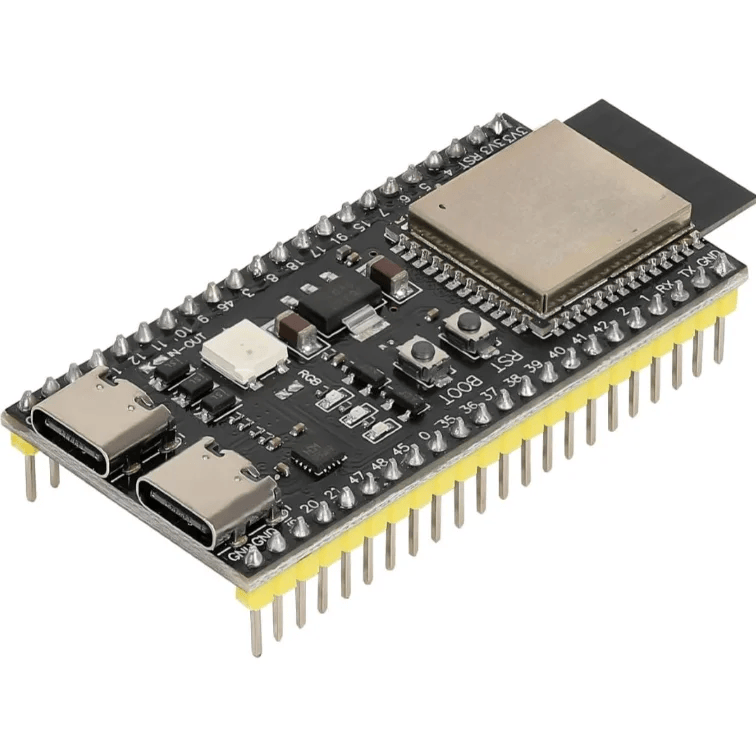
\includegraphics[width=0.45\linewidth,keepaspectratio]{gambar/gambar_2_1.png}
  \caption{Modul mikrokontroler ESP32-S3}
  \label{fig:esp32}
\end{figure}

\subsection{Modul Sensor AD8232}
\label{subsec:ad8232}

AD8232 adalah modul sensor elektrokardiogram (single-lead ECG)
yang berfungsi sebagai \textit{front-end} analog terintegrasi untuk akuisisi
sinyal biopotensial jantung. Modul ini menangkap sinyal listrik lemah dari
aktivitas jantung melalui elektroda yang ditempelkan pada tubuh pengguna,
kemudian memperkuat dan menyaring sinyal tersebut sehingga menghasilkan
keluaran analog yang bersih dan siap dicuplik oleh ADC pada
mikrokontroler~\cite{tinyml_iot_review}.

Secara internal, AD8232 mengintegrasikan penguat instrumentasi (\textit{in-amp})
\textit{low-noise}, filter \textit{high-pass} untuk menghilangkan
\textit{baseline wander}, serta filter \textit{low-pass} untuk meredam
\textit{high-frequency noise}. Hasilnya adalah sinyal ECG analog dalam rentang
0--3,3 V yang sesuai dengan level ADC ESP32-S3. Modul ini juga dilengkapi fitur
deteksi lepasnya elektroda (\textit{lead-off detection}) yang dimanfaatkan
dalam penelitian ini untuk menandai fase stabilisasi elektroda awal.

\begin{figure}[H]
  \centering
  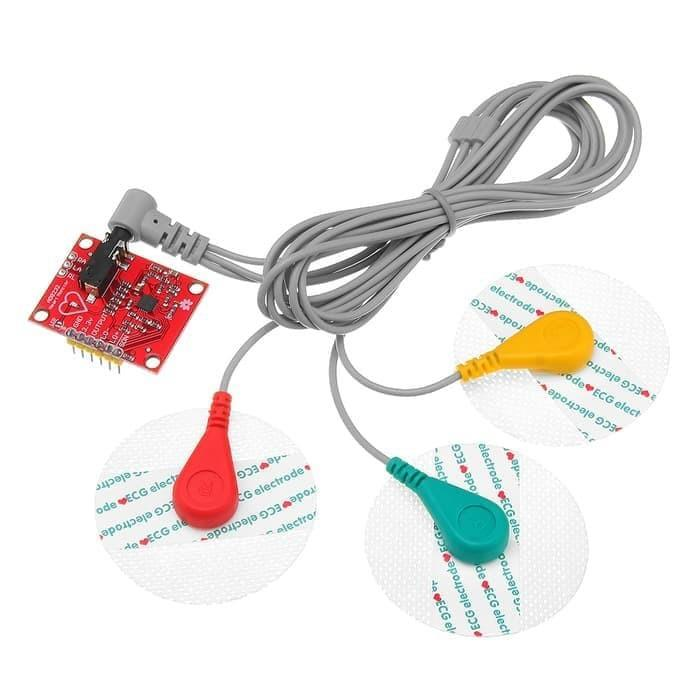
\includegraphics[width=0.55\linewidth,keepaspectratio]{gambar/gambar_2_2.png}
  \caption{Modul sensor AD8232 beserta elektroda \textit{wet-gel} tiga sadapan}
  \label{fig:ad8232}
\end{figure}

Dalam penelitian ini, AD8232 dikonfigurasi pada sadapan \textit{Modified Lead II}
(MLII) karena vektor listrik jantung sejajar dengan sudut pandang sadapan
tersebut, menghasilkan gelombang R yang paling tinggi dan paling andal untuk
deteksi R-\textit{peak} menggunakan algoritma Pan-Tompkins.

\subsection{Protokol MQTT}
\label{subsec:mqtt}

MQTT (\textit{Message Queuing Telemetry Transport}) adalah protokol komunikasi \textit{publish-subscribe} yang dirancang untuk perangkat IoT dengan \textit{overhead} \textit{header} minimal (2 byte) sehingga efisien dalam penggunaan \textit{bandwidth}~\cite{oasis_mqtt5}. MQTT mendukung tiga tingkat \textit{Quality of Service}: QoS-0 (\textit{at most once}), QoS-1 (\textit{at least once}), dan QoS-2 (\textit{exactly once}), di mana untuk data biomedis kritis seperti ECG direkomendasikan QoS-1 atau QoS-2 agar tidak ada data yang hilang saat transmisi.

\subsection{Platform Dashboard ThingsBoard}
\label{subsec:thingsboard}

ThingsBoard adalah platform IoT \textit{open-source} yang menyediakan
infrastruktur lengkap untuk pengumpulan, pemrosesan, visualisasi, dan
manajemen data perangkat IoT. Platform ini mendukung penerimaan data dari
perangkat melalui protokol MQTT secara langsung, menyimpannya dalam basis
data telemetri, dan menampilkannya melalui \textit{dashboard} yang dapat
dikonfigurasi sepenuhnya~\cite{resilient_edge_cloud}.

Dalam penelitian ini digunakan ThingsBoard Community Edition (CE) yang
dapat di-\textit{host} secara mandiri (\textit{self-hosted}). Arsitektur
ThingsBoard CE terdiri dari tiga komponen utama, yaitu \textit{broker} MQTT
terintegrasi yang menerima data telemetri dari ESP32-S3, mesin penyimpanan
telemetri berbasis \textit{time-series} untuk rekaman historis, dan
\textit{dashboard engine} berbasis WebSocket yang memperbarui tampilan secara
otomatis setiap paket baru diterima sehingga menghasilkan perilaku \textit{real-time}
dengan interval pembaruan $\approx$1 detik tanpa perlu \textit{refresh}
halaman.

\begin{figure}[H]
  \centering
  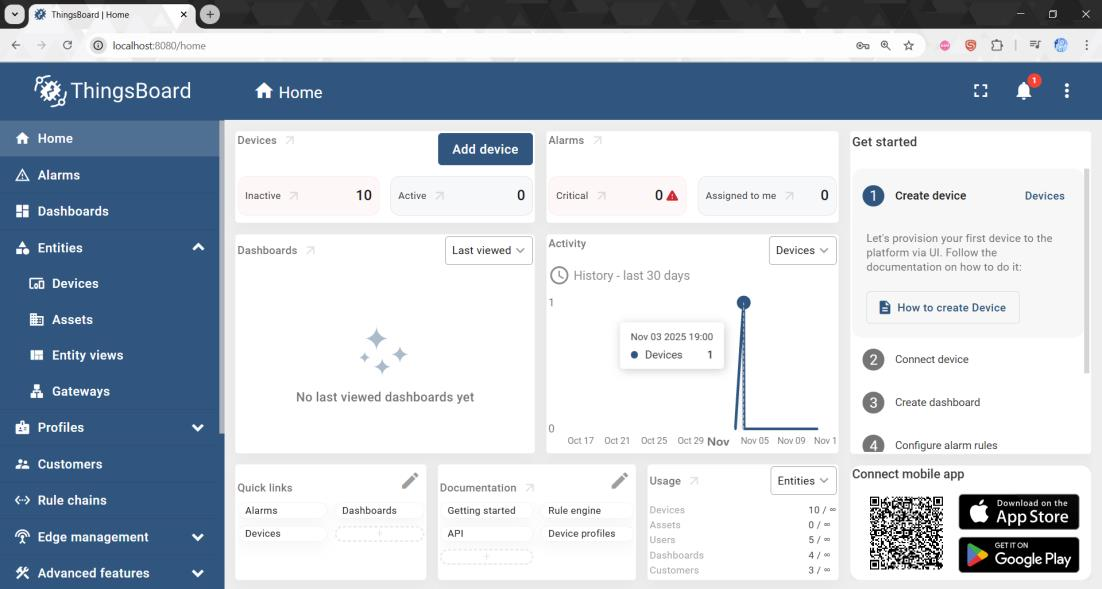
\includegraphics[width=0.92\linewidth,keepaspectratio]{gambar/gambar_2_3.png}
  \caption{Tampilan antarmuka platform ThingsBoard Community Edition}
  \label{fig:thingsboard}
\end{figure}

Sistem \textit{widget} ThingsBoard berbasis \textit{telemetry key} memungkinkan
setiap \textit{field} dalam payload JSON dari ESP32-S3 dipetakan ke komponen
visualisasi yang sesuai, seperti \textit{value card} untuk BPM, \textit{status
badge} berwarna untuk hasil klasifikasi, atau \textit{time-series chart} untuk
tren laju jantung, tanpa memerlukan pemrograman \textit{frontend} sama sekali.
ThingsBoard juga menyediakan \textit{alarm rule engine} yang dapat dikonfigurasi
untuk memicu notifikasi otomatis ketika kondisi tertentu terpenuhi, misalnya
ketika label = 1 (Aritmia terdeteksi).

\subsection{MIT-BIH \textit{Arrhythmia Database}}
\label{subsec:mitbih}

% NOTE: sloppypar dipakai karena "elektrokardiogram" bikin overfull hbox
\begin{sloppypar}
MIT-BIH \textit{Arrhythmia Database} merupakan basis data rekaman
elektrokardiogram standar yang dikembangkan melalui kolaborasi antara
Massachusetts Institute of Technology dan Beth Israel Hospital (BIH) sejak
awal tahun 1980-an. Basis data ini berisi 48 rekaman ECG dua kanal dari
47 subjek, masing-masing berdurasi sekitar 30 menit, yang dicuplik pada
frekuensi 360 Hz dengan resolusi 11-bit pada rentang $\pm$5 mV. Kanal
utama yang digunakan adalah modifikasi sadapan Lead II (MLII), yang
merupakan kanal yang sama dengan konfigurasi sensor pada penelitian
ini~\cite{moody_mark_2001}.
\end{sloppypar}

Keseluruhan rekaman telah dianotasi secara manual oleh kardiolog ahli,
menandai lokasi dan jenis setiap detak jantung. Anotasi ini menggunakan
sistem simbol standar AAMI (\textit{Association for the Advancement of
Medical Instrumentation}) yang mencakup lebih dari 15 jenis detak,
termasuk detak sinus normal (N), kontraksi ventrikular prematur (V),
dan detak supraventrikular (S). Tingkat anotasi per-detak inilah yang
menjadikan MIT-BIH sebagai \textit{benchmark} utama untuk evaluasi
algoritma deteksi aritmia secara global~\cite{moody_mark_2001}.

\begin{figure}[H]
  \centering
  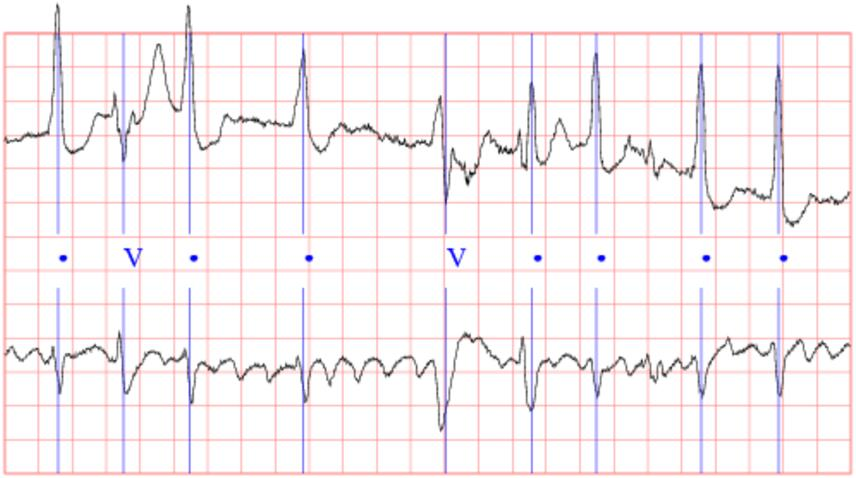
\includegraphics[width=0.90\linewidth,keepaspectratio]{gambar/gambar_2_4.png}
  \caption{Contoh visualisasi rekaman ECG dua kanal dari MIT-BIH
           \textit{Arrhythmia Database} beserta anotasi per-detak;
           simbol ``V'' menunjukkan kontraksi ventrikular prematur (PVC)
           dan simbol titik menunjukkan detak normal}
  \label{fig:mitbih-ecg}
\end{figure}

Dalam penelitian ini, MIT-BIH \textit{Arrhythmia Database} digunakan
sebagai sumber data untuk dua keperluan yang berbeda, yaitu pelatihan model CNN
menggunakan rekaman dari separuh kelompok pasien (DS1) dan pengujian
model menggunakan rekaman dari kelompok pasien yang berbeda sepenuhnya
(DS2), yang dikenal sebagai pembagian \textit{inter-patient}.
Strategi ini memastikan bahwa performa model yang diukur mencerminkan
kemampuan generalisasi terhadap pasien baru yang tidak pernah dilihat
selama pelatihan, dan bukan sekadar hafalan pola dari pasien yang sama.
Detail pemetaan anotasi menjadi label biner Normal/Aritmia diuraikan
pada Bab 3.

\section{Penelitian Terkait}
\label{sec:penelitian-terkait}

\subsection{A Multistage Denoising Framework for Ambulatory ECG Signal Based on Domain Knowledge and Motion Artifact Detection}
\label{subsec:related-xie2021}

Penelitian ini mengusulkan kerangka \textit{preprocessing} multi-tahap untuk sinyal ECG \textit{ambulatory} yang menggabungkan \textit{Frequency-Adaptive Noise Estimation} (FANE) berbasis \textit{wavelet} untuk menekan \textit{motion artifact}, \textit{Morphological Analysis and Detection} (MAD), \textit{Singular Value Thresholding} (SVT), serta \textit{Complete Ensemble Empirical Mode Decomposition} (CEEMD) untuk mengatasi \textit{baseline wander}. Kombinasi metode ini terbukti meningkatkan \textit{Signal-to-Noise Ratio} (SNR) sebesar 7\%--25\% dibandingkan metode konvensional pada \textit{dataset} ECG \textit{ambulatory}. Namun, seluruh eksperimen dilakukan pada perangkat PC server tanpa pelaporan latensi pemrosesan atau penggunaan memori. Penelitian ini memberikan referensi penting untuk memahami tantangan \textit{noise} pada ECG \textit{ambulatory}, sekaligus menunjukkan \textit{gap} bahwa algoritma \textit{preprocessing} yang efektif belum divalidasi pada MCU \textit{low-power}~\cite{xie_2021}.

\subsection{A Real-Time Embedded System to Detect QRS-Complex and Arrhythmia Classification Using LSTM Through Hybridized Features}
\label{subsec:related-karri2023}

Penelitian ini merancang sistem \textit{embedded} \textit{real-time} untuk deteksi kompleks QRS dan klasifikasi aritmia menggunakan pendekatan \textit{hybrid} yang menggabungkan \textit{Discrete Wavelet Transform} (DWT), \textit{Delta-Sigma Modulation} (DSM), dan model LSTM. Sistem DWT+DSM mampu mendeteksi kompleks QRS dalam 17,2 ms dengan konsumsi daya 680 nW pada chip DSM, dan diuji pada Raspberry Pi 4 (ARM Cortex-A72, RAM 4 GB). Meskipun berhasil menunjukkan kelayakan pemrosesan ECG secara \textit{embedded}, penggunaan Raspberry Pi 4 tidak mewakili batasan MCU \textit{low-power} yang sesungguhnya. \textit{Gap} pada penelitian ini adalah absennya implementasi dan validasi pada MCU kelas ESP32 atau Cortex-M4~\cite{karri_2023}.

\subsection{Real-Time Fetal Arrhythmia Detection Using Deep Learning on an Embedded fECG Monitoring System}
\label{subsec:related-mekhfioui2025}

Penelitian ini mengembangkan sistem deteksi aritmia jantung janin berbasis sinyal fECG menggunakan \textit{Independent Component Analysis} (ICA) untuk separasi sinyal, diikuti \textit{bandpass filtering} dan segmentasi ke dalam jendela 3 detik, serta klasifikasi menggunakan model 1D-CNN ringan yang diimplementasikan pada Raspberry Pi. Sistem mencapai akurasi 98,2\%, sensitivitas 98,8\%, dan F1-\textit{score} 98,1\% pada \textit{dataset} Kaggle dan NIFECGDB. Penelitian ini menjadi acuan arsitektur 1D-CNN untuk klasifikasi sinyal kardiovaskular pada \textit{embedded system}, namun implementasinya masih pada Raspberry Pi dan ICA belum dievaluasi pada MCU dengan batasan RAM dan daya yang jauh lebih ketat~\cite{mekhfioui_2025}.

\subsection{TinyML-Based Classification in an ECG Monitoring Embedded System}
\label{subsec:related-kim2023}

Penelitian ini mengusulkan TinyCES, sebuah model 1D-CNN terkuantisasi yang dirancang khusus untuk monitoring ECG pada perangkat \textit{embedded} dengan sumber daya sangat terbatas. Model berhasil di-\textit{deploy} pada Arduino Nano 33 BLE Sense (ARM Cortex-M4) dengan ukuran model 27 KB dan akurasi klasifikasi biner sebesar 97\% menggunakan \textit{dataset} MIT-BIH dan PTB ECG. Penelitian ini merupakan salah satu dari sedikit studi yang benar-benar menjalankan inferensi ECG di MCU fisik \textit{low-power}. Namun, TinyCES masih terbatas pada klasifikasi biner dan tidak menyertakan laporan latensi inferensi, penggunaan RAM saat \textit{runtime}, maupun konsumsi daya aktual selama operasi kontinu~\cite{kim_2023}.

\subsection{Designing Resilient IoT and Edge Computing with Federated TinyML}
\label{subsec:related-laiu2026}

Penelitian ini mengusulkan arsitektur DRIFT (\textit{Distributed Resilient IoT Federated TinyML}), sebuah kerangka tiga-lapisan yang mengintegrasikan TinyML dan \textit{Federated Learning} untuk meningkatkan keamanan dan ketahanan sistem IoT/MCU. Penelitian ini menunjukkan bahwa kuantisasi float32 ke INT8 menghasilkan kompresi model $4\times$ dengan degradasi akurasi kurang dari $0{,}01\%$, serta membuktikan bahwa beban komputasi pada MCU dapat dikurangi melalui \textit{preprocessing} terdistribusi di lapisan \textit{edge}. Fokus penelitian ini adalah pada keamanan siber IoT, bukan pada monitoring sinyal biomedis, dan evaluasinya dilakukan secara simulasi tanpa pengujian \textit{streaming} data ECG kontinu pada \textit{hardware} MCU fisik~\cite{laiu_2026}.

\subsection{Implementing TinyML in Internet of Things Devices: A Systematic Literature Review}
\label{subsec:related-solispino2026}

Penelitian ini melakukan tinjauan literatur sistematis terhadap 114 studi primer tentang implementasi TinyML pada perangkat IoT menggunakan protokol PRISMA dan strategi pencarian multi-\textit{database}. Hasil \textit{review} mengungkapkan bahwa CNN adalah arsitektur yang paling sering digunakan, ESP32 dan Arduino Nano 33 BLE Sense adalah platform \textit{hardware} yang paling umum, serta \textit{healthcare} adalah domain aplikasi yang paling banyak diteliti. Tinjauan ini juga mengidentifikasi tantangan utama yang belum terselesaikan, meliputi keterbatasan memori/CPU, kerentanan keamanan, dan absennya standardisasi implementasi TinyML antar platform. Penelitian ini memberikan landasan komprehensif untuk pemilihan \textit{framework} dan platform pada penelitian ini~\cite{tinyml_iot_review}.

\subsection{Advanced IoT-Enabled Embedded Wearable System for Continuous Cardiovascular Health Monitoring Using Edge Intelligence}
\label{subsec:related-sheebarani2026}

Penelitian ini mengusulkan sistem \textit{wearable} monitoring kardiovaskular kontinu yang mengimplementasikan model \textit{hybrid} 1D-TA-DSC (kombinasi 1D \textit{Depthwise Separable Convolution} dan \textit{Temporal Attention}-GRU) pada ARM Cortex-M4 menggunakan TFLite. Setelah kuantisasi \textit{post-training}, model dikompres dari 22 KB menjadi 11 KB dengan latensi inferensi 7 ms, akurasi 99,8\%, dan AUROC 0,997 pada \textit{dataset} MIMIC-III (rekaman ICU). Penelitian ini adalah salah satu yang paling detail dalam melaporkan metrik \textit{hardware} untuk monitoring kardiovaskular di MCU, namun tidak menyertakan evaluasi konsumsi daya pada kondisi operasi kontinu maupun mekanisme resiliensi \textit{pipeline} \textit{edge-to-cloud}~\cite{sheeba_rani_2026}.

\subsection{An On-Device Machine Learning Assisted System for Unobtrusive Cardiac Auscultation}
\label{subsec:related-chowdhury2023}

Penelitian ini mengembangkan sistem auskultasi jantung berbasis \textit{on-device machine learning} yang diimplementasikan pada Arduino Nano 33 BLE Sense (ARM Cortex-M4, 64 MHz) untuk klasifikasi suara jantung secara \textit{real-time} tanpa koneksi internet. Sistem melaporkan latensi \textit{pipeline} DSP sebesar 23,19 ms untuk ekstraksi fitur MFCC, dengan konsumsi arus puncak 8,6 mA pada 3,3 V (sekitar 28,38 mW) dan daya tahan baterai 11,5 jam menggunakan baterai 240 mAh. Penelitian ini memberikan referensi \textit{benchmark} konsumsi daya aktual untuk \textit{inference on-device} pada MCU Cortex-M4, meskipun fokusnya pada auskultasi suara jantung, bukan sinyal ECG~\cite{chowdhury_2023}.

\subsection{AI-Powered Anomaly Detection and Cybersecurity in Healthcare IoT with Fog/Edge}
\label{subsec:related-alquayed2026}

Penelitian ini mengusulkan kerangka FE-ACS yang mendistribusikan pemrosesan dan deteksi anomali ke lapisan \textit{fog} dan \textit{edge} pada ekosistem IoT kesehatan. Pengukuran performa menunjukkan bahwa arsitektur \textit{fog-edge} mencapai latensi total rata-rata 18,7 ms dibandingkan 152,3 ms pada arsitektur \textit{cloud-centric}, mempresentasikan peningkatan 87,7\% dengan efisiensi \textit{bandwidth} $8{,}5\times$ lebih tinggi. Penelitian ini membuktikan secara kuantitatif keunggulan arsitektur \textit{edge} atas \textit{cloud-centric} untuk aplikasi IoT kesehatan. Namun, fokus penelitian ini adalah pada keamanan siber, bukan pada \textit{streaming} data ECG kontinu, dan tidak membahas mekanisme resiliensi saat koneksi terputus~\cite{al_quayed_2026}.

\subsection{Resilient Edge-to-Cloud Architecture with Self-Healing and Self-Correcting Mechanisms for Industrial Data Continuity}
\label{subsec:related-boluda2026}

Penelitian ini mengusulkan arsitektur E2C (\textit{Edge-to-Cloud}) berbasis \textit{microservices} dengan mekanisme \textit{self-healing} dan \textit{self-correcting} menggunakan \textit{stack} Kubernetes, Rancher, Prometheus, Grafana, dan Node-RED. Sistem menggunakan MQTT sebagai protokol transmisi dengan mekanisme \textit{edge buffering} yang mempertahankan \textit{Recovery Point Objective} (RPO) mendekati nol untuk aliran data kritis saat terjadi saturasi jaringan. Pengujian \textit{stress test} dengan kondisi \textit{overload} CPU dan saturasi jaringan menunjukkan kemampuan sistem mendeteksi \textit{threshold}, melakukan \textit{scaling}, dan mengisolasi \textit{node} bermasalah secara otomatis. Meskipun prinsip resiliensi pada penelitian ini relevan untuk \textit{streaming} ECG, seluruh implementasi berfokus pada data \textit{time-series} industri manufaktur dan menggunakan infrastruktur berbasis Kubernetes yang terlalu berat untuk MCU \textit{low-power}~\cite{resilient_edge_cloud}.

\subsection{Real-Time Cardiac Arrhythmia Classification Using TinyML on
Ultra-Low-Cost Microcontrollers}
\label{subsec:related-zambrano2026}

Penelitian ini mendemonstrasikan klasifikasi aritmia \emph{real-time} menggunakan
1D-CNN terkuantisasi INT8 yang di-\emph{deploy} pada mikrokontroler Arduino UNO 8-bit
(ATmega328P, SRAM 2 KB, Flash 32 KB). Sistemnya mengintegrasikan akuisisi sinyal ECG
dengan \emph{front-end} analog AD8232, filter Butterworth \emph{bandpass} 0,5--40 Hz,
deteksi R-peak Pan-Tompkins, segmentasi \emph{window} 250 sampel (sekitar 0,7 detik
pada 360 Hz), hingga visualisasi pada layar OLED. Model dilatih dan dievaluasi pada
MIT-BIH Arrhythmia Database untuk tiga kelas (Normal, Ventrikular, Supraventrikular),
menghasilkan model berukuran di bawah 22 KB dengan latensi inferensi sekitar 200 ms
per detak dan degradasi akurasi kurang dari 0,7\% akibat kuantisasi INT8. Validasi
dilakukan melalui dua jalur terpisah, yaitu evaluasi model pada dataset \emph{benchmark}
dan uji fungsional \emph{real-time} menggunakan relawan sehat tanpa penegakan diagnosis
klinis. Penelitian ini memberikan bukti kelayakan bahwa pipeline
akuisisi--preprocessing--inferensi INT8 dapat berjalan pada mikrokontroler yang
jauh lebih terbatas dari ESP32-S3. Namun, pembagian datanya dilakukan per-detak tanpa
pemisahan antarpasien, sehingga metriknya berpotensi optimistis. Penelitian yang
diusulkan justru mengadopsi skema antarpasien (inter-patient, DS1/DS2) yang lebih ketat
untuk mengukur generalisasi~\cite{zambrano_2026}.

\subsection{Rancang Bangun Smart Wearables Terintegrasi IoT untuk Deteksi Dini
Atrial Fibrilasi Menggunakan SVM Berbasis Cloud}
\label{subsec:related-mulyawan2026}

Penelitian ini merancang perangkat \emph{wearable} berbasis ESP32 yang mengintegrasikan
sensor EKG AD8232, sensor SpO\textsubscript{2} MAX30102, dan sensor suhu MLX90614 untuk
deteksi dini atrial fibrilasi (AFib). Deteksi puncak R dan ekstraksi fitur interval RR
dilakukan di sisi \emph{edge}, kemudian fitur ditransmisikan via MQTT ke infrastruktur
\emph{cloud} lokal berbasis ThingsBoard Community Edition dan basis data PostgreSQL.
Klasifikasi dilakukan oleh model Support Vector Machine (SVM) dengan kernel Radial Basis
Function yang \emph{di-deploy pada sisi backend}, dilatih menggunakan dataset MIT-BIH dan
mencapai akurasi tinggi pada pengujian \emph{offline}~\cite{mulyawan_2026}.
Gambar~\ref{fig:alat-mulyawan} menampilkan \emph{prototype} perangkat yang dihasilkan.

\begin{figure}[H]
  \centering
  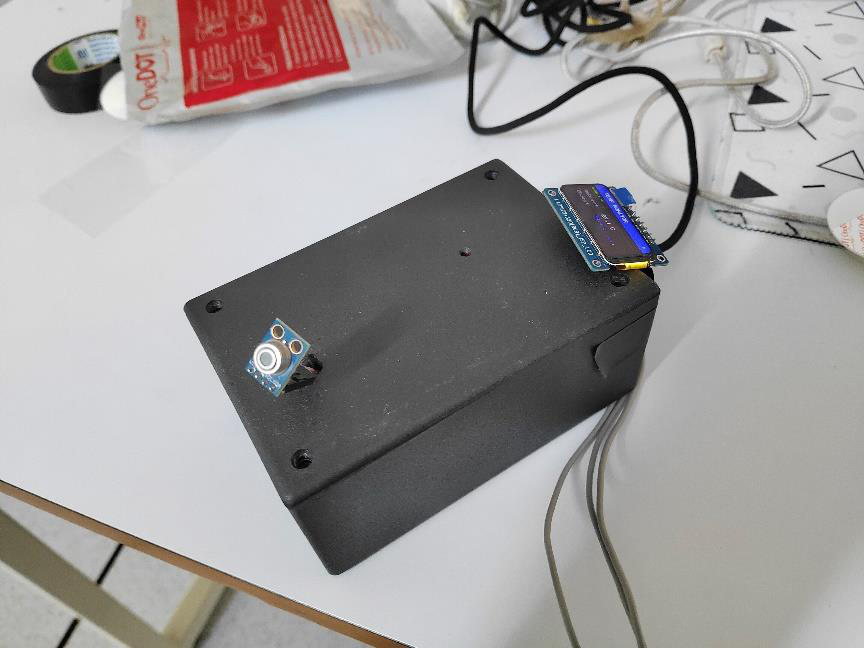
\includegraphics[width=0.7\linewidth]{gambar/gambar_alat_terdahulu_mulyawan.png}
  \caption{\emph{Prototype} perangkat \emph{wearable} pada penelitian
  terdahulu~\cite{mulyawan_2026}: integrasi ESP32 dan sensor AD8232/MAX30102/MLX90614 dalam \emph{blackbox}}
  \label{fig:alat-mulyawan}
\end{figure}

Penelitian ini merupakan pendahulu langsung dari penelitian yang diusulkan, menggunakan
platform sensor dan \emph{dashboard} yang sama. Perbedaan mendasarnya terletak pada
lokasi inferensi. Pada penelitian sebelumnya, klasifikasi dijalankan secara terpusat di \emph{cloud} sehingga
pengambilan keputusan tetap bergantung pada ketersediaan koneksi, sedangkan penelitian
ini memindahkan inferensi sepenuhnya ke perangkat (\emph{on-device}) menggunakan CNN
terkuantisasi INT8. Selain itu, penelitian terdahulu juga belum menyertakan mekanisme
resiliensi \emph{pipeline} saat koneksi terputus.

\subsection{Perbandingan Penelitian Terkait}
\label{subsec:perbandingan-penelitian}

Berdasarkan ulasan kedua belas penelitian di atas, Tabel~\ref{tab:perbandingan-penelitian} merangkum perbandingan metode, platform, dan \textit{gap} dari masing-masing penelitian.

{\scriptsize
\setlength{\tabcolsep}{3pt}
\renewcommand{\arraystretch}{1.2}
\begin{longtable}{|c|L{3.5cm}|L{2.0cm}|L{2.0cm}|L{1.8cm}|L{2.8cm}|}
\caption{Perbandingan Penelitian Terkait}\label{tab:perbandingan-penelitian}\\
\hline
\rowcolor{headgray}
\textbf{No} & \textbf{Judul (Tahun)} & \textbf{Penyakit / Domain} & \textbf{Metode (Model)} & \textbf{Platform Komputasi} & \textbf{Perbedaan} \\ \hline
\endfirsthead

\hline
\rowcolor{headgray}
\textbf{No} & \textbf{Judul (Tahun)} & \textbf{Penyakit / Domain} & \textbf{Metode (Model)} & \textbf{Platform Komputasi} & \textbf{Perbedaan} \\ \hline
\endhead

\hline
\endfoot

\hline
\endlastfoot

1 & \textit{A multi-stage denoising framework for ambulatory ECG signal based on domain knowledge and motion artifact detection} (2021) & Preprocessing sinyal ECG (penekanan noise) & FANE+MAD, SVT, CEEMD, wavelet (denoising bertingkat) & PC server (offline) & Efektif menekan \textit{motion artifact} ambulatory (SNR naik 7--25\%), namun hanya dievaluasi di PC server dan beban CEEMD berat; belum diuji maupun dikuantisasi pada mikrokontroler hemat daya. \\ \hline

2 & \textit{A real-time embedded system to detect QRS-complex and arrhythmia classification using LSTM through hybridized features} (2023) & Aritmia & DWT + Delta-Sigma Modulation + LSTM & Raspberry Pi 4 & Akurasi tinggi (99,6\%) dan sudah \textit{real-time} di \textit{embedded}, tetapi Raspberry Pi bukan MCU kelas ESP32/Cortex-M4; daya total dan RAM tidak diukur, serta tanpa integrasi cloud. \\ \hline

3 & \textit{Real-time fetal arrhythmia detection using deep learning on an embedded fECG monitoring system} (2025) & Aritmia janin (\textit{fetal}) & Bandpass + ICA + 1D-CNN ringan & Raspberry Pi 4 & Memakai 1D-CNN ringan dengan transmisi Wi-Fi, namun tetap di Raspberry Pi (bukan MCU \textit{low-power}); ICA sensitif noise dan belum dievaluasi di MCU, serta konsumsi daya baterai tidak dilaporkan. \\ \hline

4 & \textit{TinyML-Based Classification in an ECG Monitoring Embedded System} (2023) & Aritmia (klasifikasi biner normal/\allowbreak abnormal) & 1D-CNN INT8 (TFLM, \textit{Post-Training Quantization}) & Arduino Nano BLE (Cortex-M4) & Inferensi \textit{on-device} INT8 (\textasciitilde27 KB, akurasi \textasciitilde97\%)---paling dekat dengan pendekatan ini---tetapi terbatas klasifikasi biner; latensi inferensi dan konsumsi daya tidak dilaporkan, serta tanpa pipeline \textit{edge-to-cloud} yang resilien. \\ \hline

5 & \textit{Designing resilient IoT and Edge Computing with federated TinyML} (2026) & --- (keamanan jaringan IoT) & \textit{Federated Learning} + kuantisasi MLP INT8 & Testbed/\allowbreak simulasi & Membuktikan kuantisasi float32$\rightarrow$INT8 (kompresi 4$\times$, akurasi turun $<$0,01\%), tetapi domainnya deteksi intrusi jaringan---bukan \textit{streaming} ECG---dan belum ada \textit{benchmark} inferensi di MCU fisik. \\ \hline

6 & \textit{Implementing TinyML in Internet of Things devices: A systematic literature review} (2026) & --- (tinjauan literatur, 114 studi) & SLR (PRISMA) & Berbagai (MCU + SBC) & Memetakan algoritma, hardware, dan tantangan TinyML secara komprehensif, namun bukan studi eksperimental; menyoroti belum adanya standardisasi implementasi TinyML serta keterbatasan memori/CPU. \\ \hline

7 & \textit{Advanced IoT-enabled embedded wearable system for continuous cardiovascular health monitoring using edge intelligence} (2026) & Penyakit kardio\-vaskular / aritmia (4 kelas keparahan) & 1D Depthwise-\allowbreak Separable Conv + Temporal Attention-\allowbreak GRU (INT8 PTQ) & ARM Cortex-M4 (STM32\-F407) & Inferensi sangat cepat (\textasciitilde7 ms) dengan model kecil (\textasciitilde11 KB) di Cortex-M4, namun tidak melaporkan resiliensi pipeline \textit{edge-to-cloud} dan dilatih pada data ICU (MIMIC-III) yang belum tentu \textit{generalize} ke kondisi ambulatory. \\ \hline

8 & \textit{An on-device machine learning assisted system for unobtrusive cardiac auscultation} (2023) & Kelainan jantung (auskultasi/\allowbreak PCG) & DSP + MFCC + ML \textit{on-device} & Arduino Nano BLE & Berhasil menjalankan ML \textit{on-device}, tetapi memproses sinyal suara jantung (PCG), bukan sinyal ECG. \\ \hline

9 & \textit{AI-Powered Anomaly Detection and Cybersecurity in Healthcare IoT with Fog/Edge} (2026) & Keamanan siber IoT kesehatan & Kerangka FE-ACS (deteksi anomali \textit{fog-edge}) & Arsitektur \textit{fog/edge} IoT & Membuktikan keunggulan latensi \textit{fog-edge} (18,7 ms vs 152,3 ms), tetapi berfokus pada keamanan siber---bukan \textit{streaming} ECG kontinu---dan tanpa mekanisme resiliensi saat koneksi terputus. \\ \hline

10 & \textit{Resilient Edge-to-Cloud Architecture with Self-Healing and Self-Correcting Mechanisms for Industrial Data Continuity} (2026) & Kontinuitas data industri & E2C \textit{microservices} + MQTT + \textit{edge buffering} (\textit{self-healing}) & Kubernetes (Rancher, Prometheus, Grafana) & Resiliensi RPO mendekati nol saat saturasi jaringan relevan untuk \textit{streaming} ECG, namun berfokus pada data \textit{time-series} industri dan memakai Kubernetes yang terlalu berat untuk MCU \textit{low-power}. \\ \hline

11 & \textit{Real-Time Cardiac Arrhythmia Classification Using TinyML on Ultra-Low-Cost Microcontrollers} (2026) & Aritmia (3 kelas: N/V/S) & 1D-CNN INT8 (TFLM, PTQ) + AD8232 & Arduino UNO 8-bit (ATmega328P) & Membuktikan pipeline AD8232 $\rightarrow$ preprocessing $\rightarrow$ inferensi INT8 jalan di MCU sangat terbatas (SRAM 2 KB, model $<$22 KB), tetapi pembagian data per-detak (bukan inter-patient) sehingga metrik berpotensi optimistis; tanpa cabang ritme RR maupun pipeline edge-to-cloud resilien. \\ \hline

12 & \textit{Rancang Bangun Smart Wearables Terintegrasi IoT untuk Deteksi Dini Atrial Fibrilasi Menggunakan SVM Berbasis Cloud} (2026) & Atrial fibrilasi & Fitur RR + SVM (RBF) & ESP32 (akuisisi) + SVM di cloud & Pendahulu langsung dengan sensor \& dashboard sama, tetapi inferensi terpusat di cloud (bukan on-device); tanpa kuantisasi model di MCU dan tanpa mekanisme resiliensi pipeline saat koneksi terputus. \\ \hline

13 & \textit{Implementasi Sistem Monitoring Detak Jantung Kontinu Berbasis IoT Edge Computing untuk Deteksi Dini Aritmia} (Proposed System) & Aritmia (deteksi dini) & \textit{Preprocessing} di MCU (Butterworth + Pan-Tompkins) + 1D-CNN INT8 + fitur RR (\textit{hybrid}) \textit{on-device} ($<$20 KB) & \textit{ESP32-S3 (inferensi on-device)} & Menyatukan preprocessing \textit{real-time} di MCU, inferensi CNN INT8 langsung di perangkat, dan pipeline \textit{edge-to-cloud} resilien (\textit{ring-buffer} lokal + MQTT) dalam satu perangkat ESP32-S3 hemat daya. \\ \hline

\end{longtable}
}

Dari Tabel~\ref{tab:perbandingan-penelitian} terlihat bahwa belum ada penelitian yang secara komprehensif mengintegrasikan ketiga aspek sekaligus, yaitu algoritma \textit{preprocessing} ECG yang divalidasi di MCU \textit{low-power}, inferensi TinyML \textit{on-device} pada ESP32-S3, serta pipeline \textit{edge-to-cloud} dengan mekanisme resiliensi berbasis MQTT \textit{local buffering}.
